\documentclass[11pt]{article}

\usepackage{verbatim}
\usepackage{amsmath}
\usepackage{amssymb}
\usepackage{setspace}
\usepackage[top=1in, bottom=1in, left=1.25in, right=1.25in]{geometry}
\usepackage{subfigure}
\usepackage{graphicx}
\usepackage{cite}
\usepackage[squaren]{SIunits}
\usepackage{listings}

\setlength{\parindent}{0pt} 	% remove the silly paragraph indents

\begin{document}



% ---------------------------------------
% Name section
% ---------------------------------------
\begin{flushleft}
Sherman Lam
\\E155
\\ \today
\end{flushleft}


% ---------------------------------------
% Title
% ---------------------------------------
\begin{center}
\begin{Large}
\textbf{Lab 3 Report: Keypad Scanner}
\end{Large}
\end{center}


% ---------------------------------------
% Start report
% ---------------------------------------


\section{Introduction}
\label{sec:intro}

In this lab, I used created an interface between a keypad and the dual-display system developed in Lab 2. When a number is pressed on the key pad, the number is recorded on the 2 displays. The most recently pressed number is shown on the "right" display (closer to the bottom of the board). The second most recently pressed number is shown on the "left" display (close to the top of the board). Figure \ref{fig:board} illustrates an example where "42" was entered into the keypad.

\begin{figure}[h!]
\centering
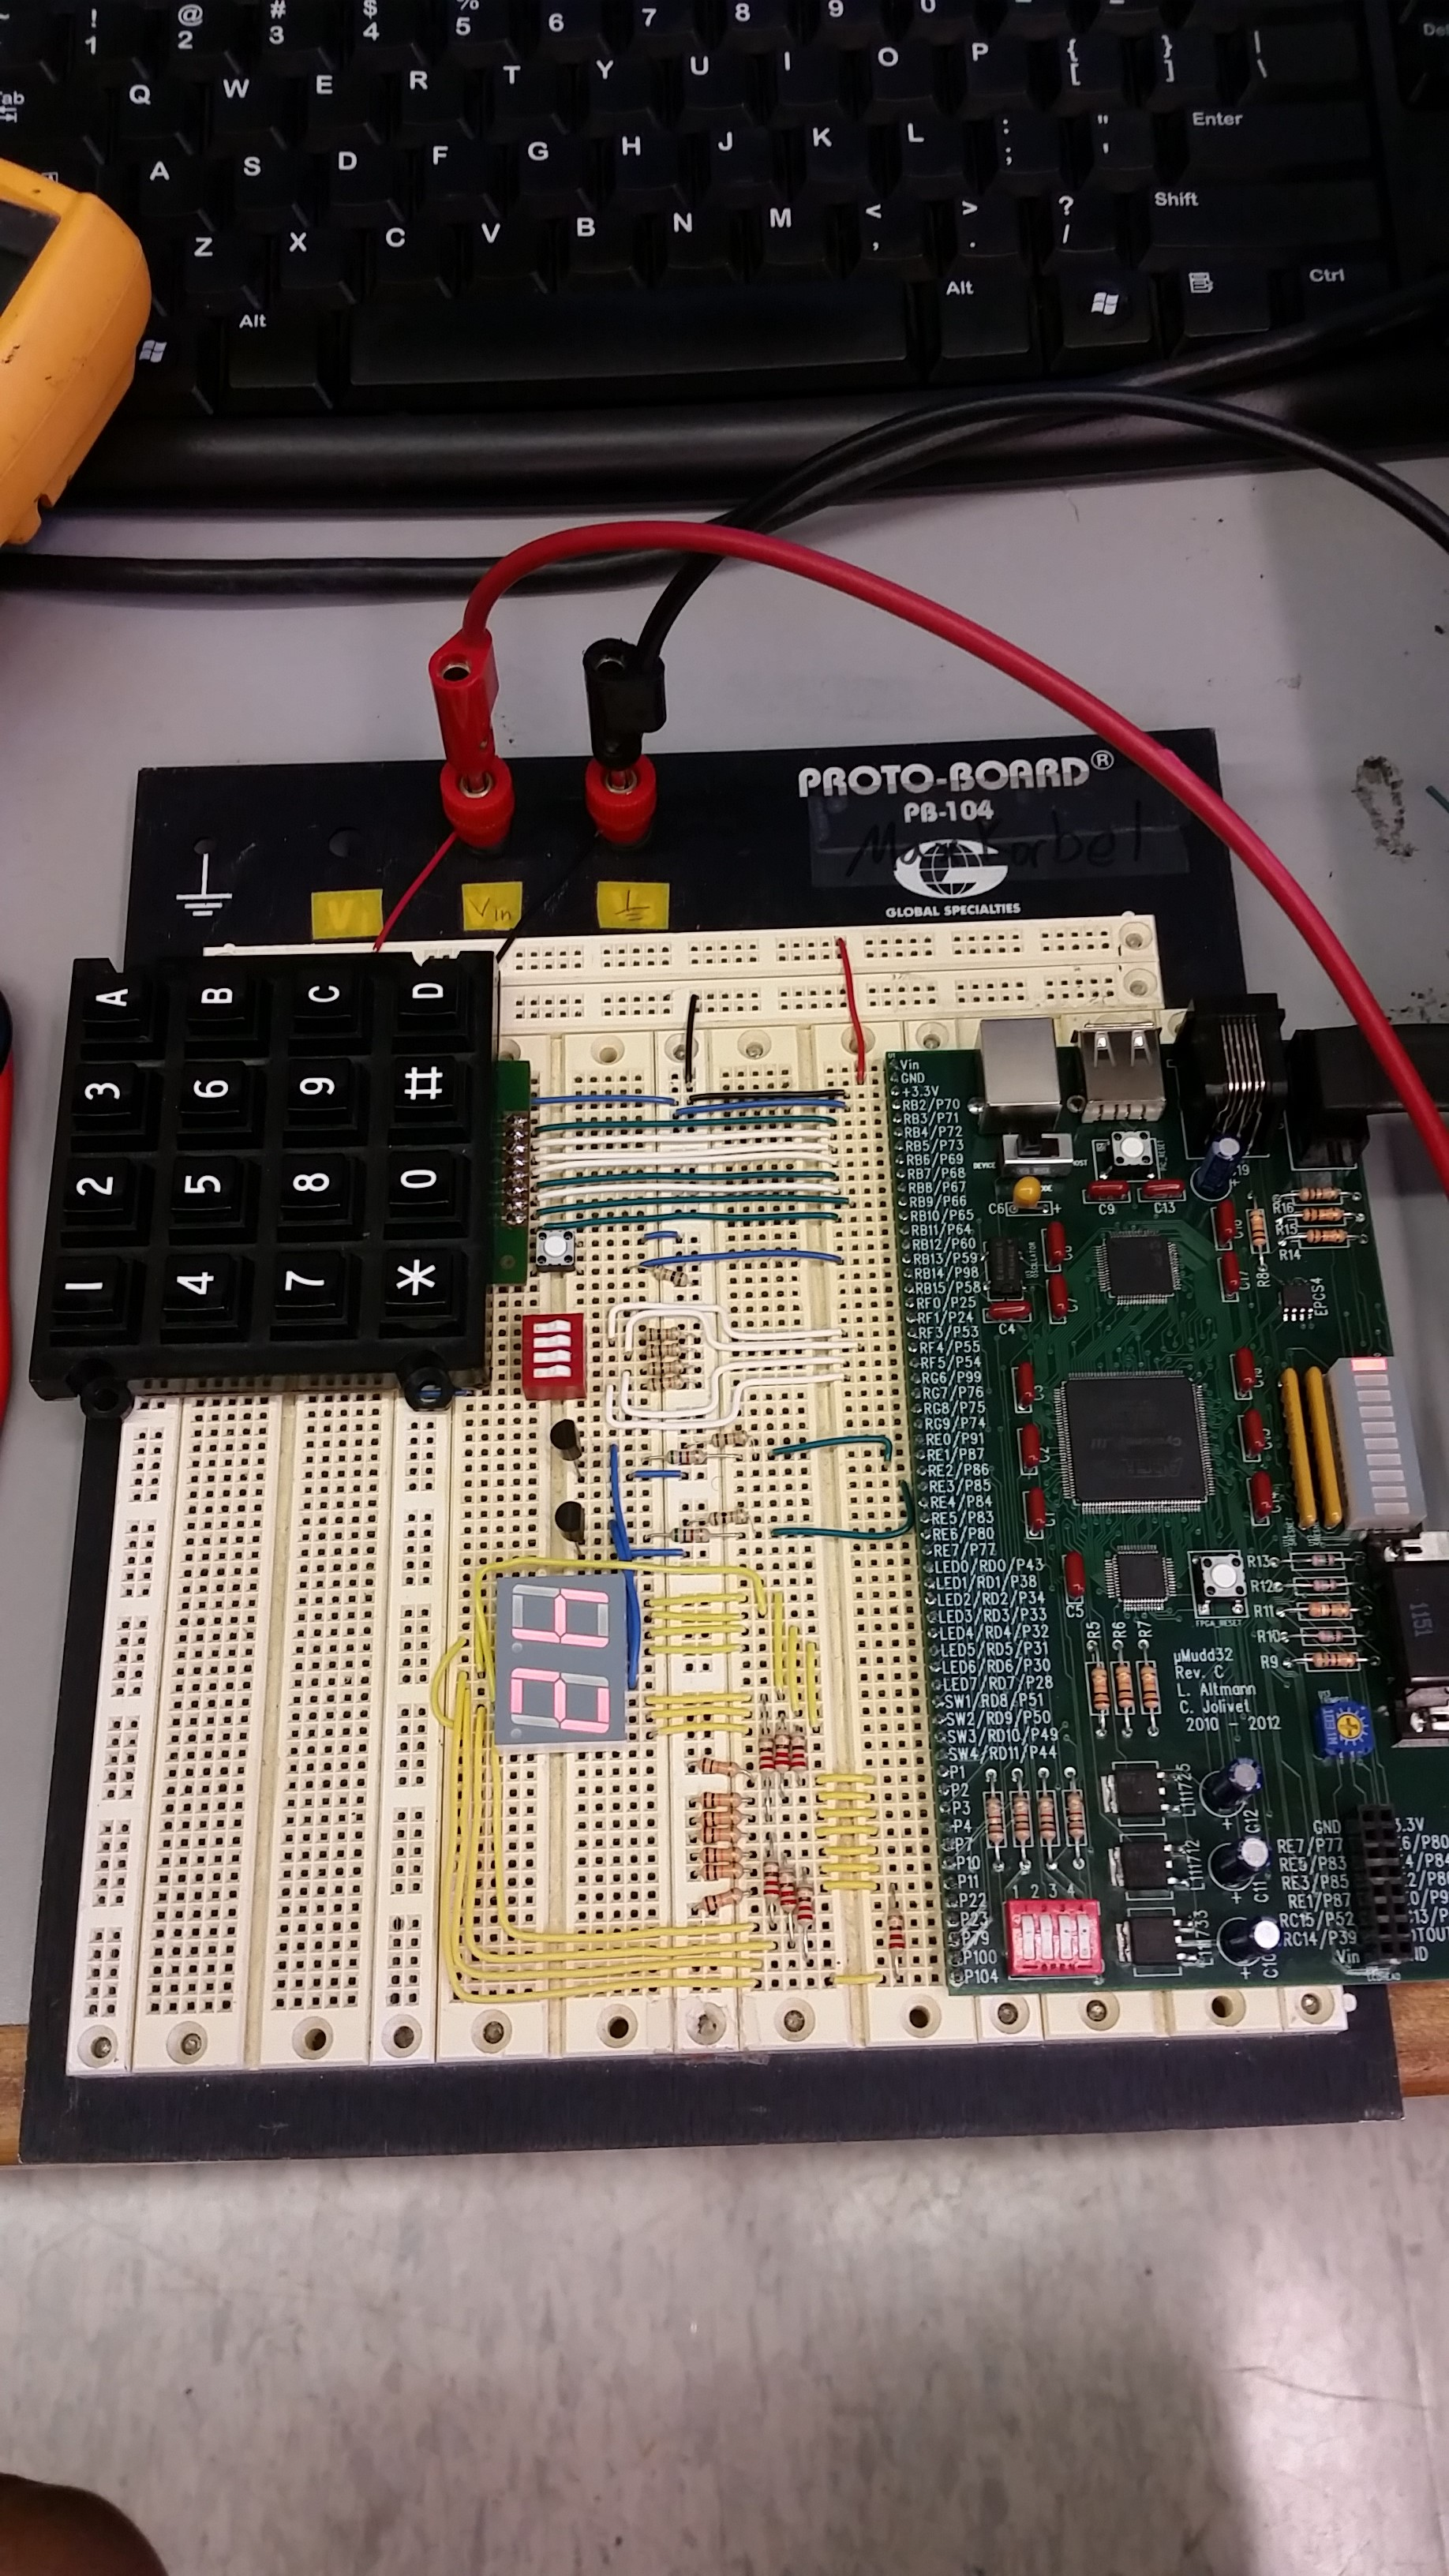
\includegraphics[scale=0.11]{board.jpg}
\caption{The latest number entered on the keypad is displayed on the bottom display. The second latest number is displayed on the top.}
\label{fig:board}
\end{figure} 


\section{Design and Testing Methodology}

\subsection{Hardware}

The keypad has 4 rows and 4 columns, which allows me to represent all 16 hex values (see Figure \ref{fig:keypad_pinout}. When a particular button is pressed its row and column are connected. For example, the button for the number 5 is on row 1 and column 1. When that button is pressed, row 1 and col 1 will be in contact. If pin R1 was pulled to HIGH, pin C1 would also register a HIGH. \\

To detect which button is pressed, each row is powered individually. Then the logic levels of the columns are read to determine if any buttons are pressed. Since the rows are being powered, they will always resolve to HIGH or LOW. However, to ensure that the columns also resolve to a logic level, pull-down resistors are placed on the column pins (C0 - C3). In this configuration, if a button is pressed, it will read HIGH, otherwise it will read low (See Figure \ref{fig:keypad_sch}). \\


\begin{figure}[h!]
\centering
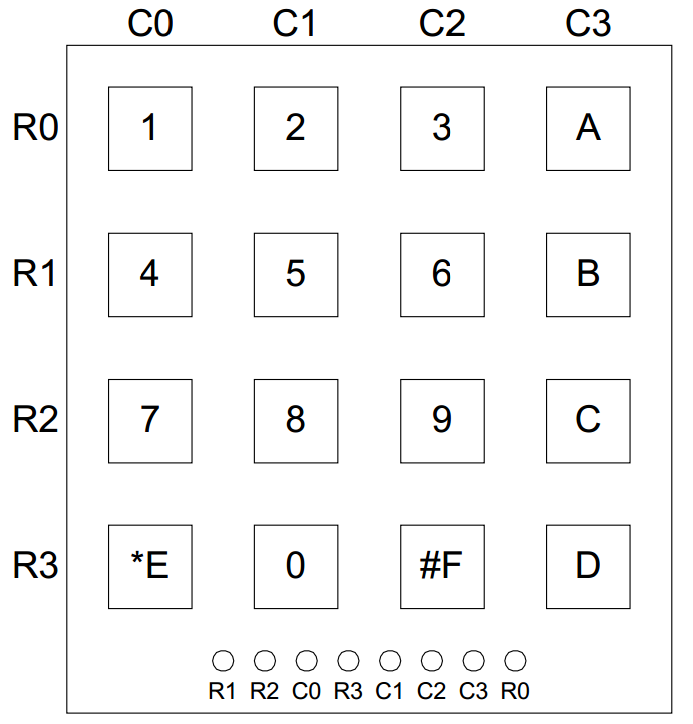
\includegraphics[scale=0.35]{keypad_pinout.png}
\caption{Pinout and key layout of the keypad. Image obtained from the HMC, E155 lab page.}
\label{fig:keypad_pinout}
\end{figure} 

\begin{figure}[h!]
\centering
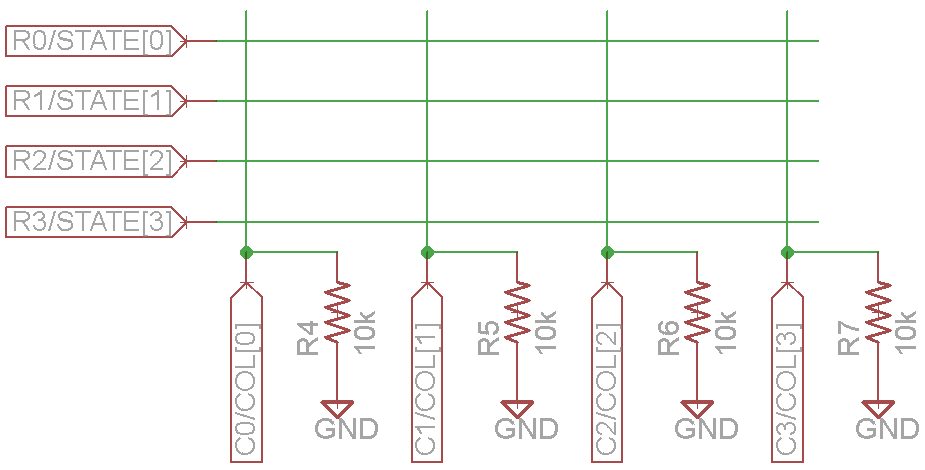
\includegraphics[scale=0.4]{keypad_sch.png}
\caption{Schematic representation of the keypad. When a button is pressed, its row and col are connected.}
\label{fig:keypad_sch}
\end{figure} 


\subsection{Button Bounce}
\label{sec:button_bounce}

One of the challenges with using the keypad is a phenomenon known as "button bounce." This occurs because when a mechanical button is pressed and released, the button continues to move up and down for a short duration of time. This in turn causes the contact to close and open. Figures \ref{fig:bounce_rise} and \ref{fig:bounce_fall} show button bounce as viewed from an oscilloscope. \\


\begin{figure}[h!]
\centering
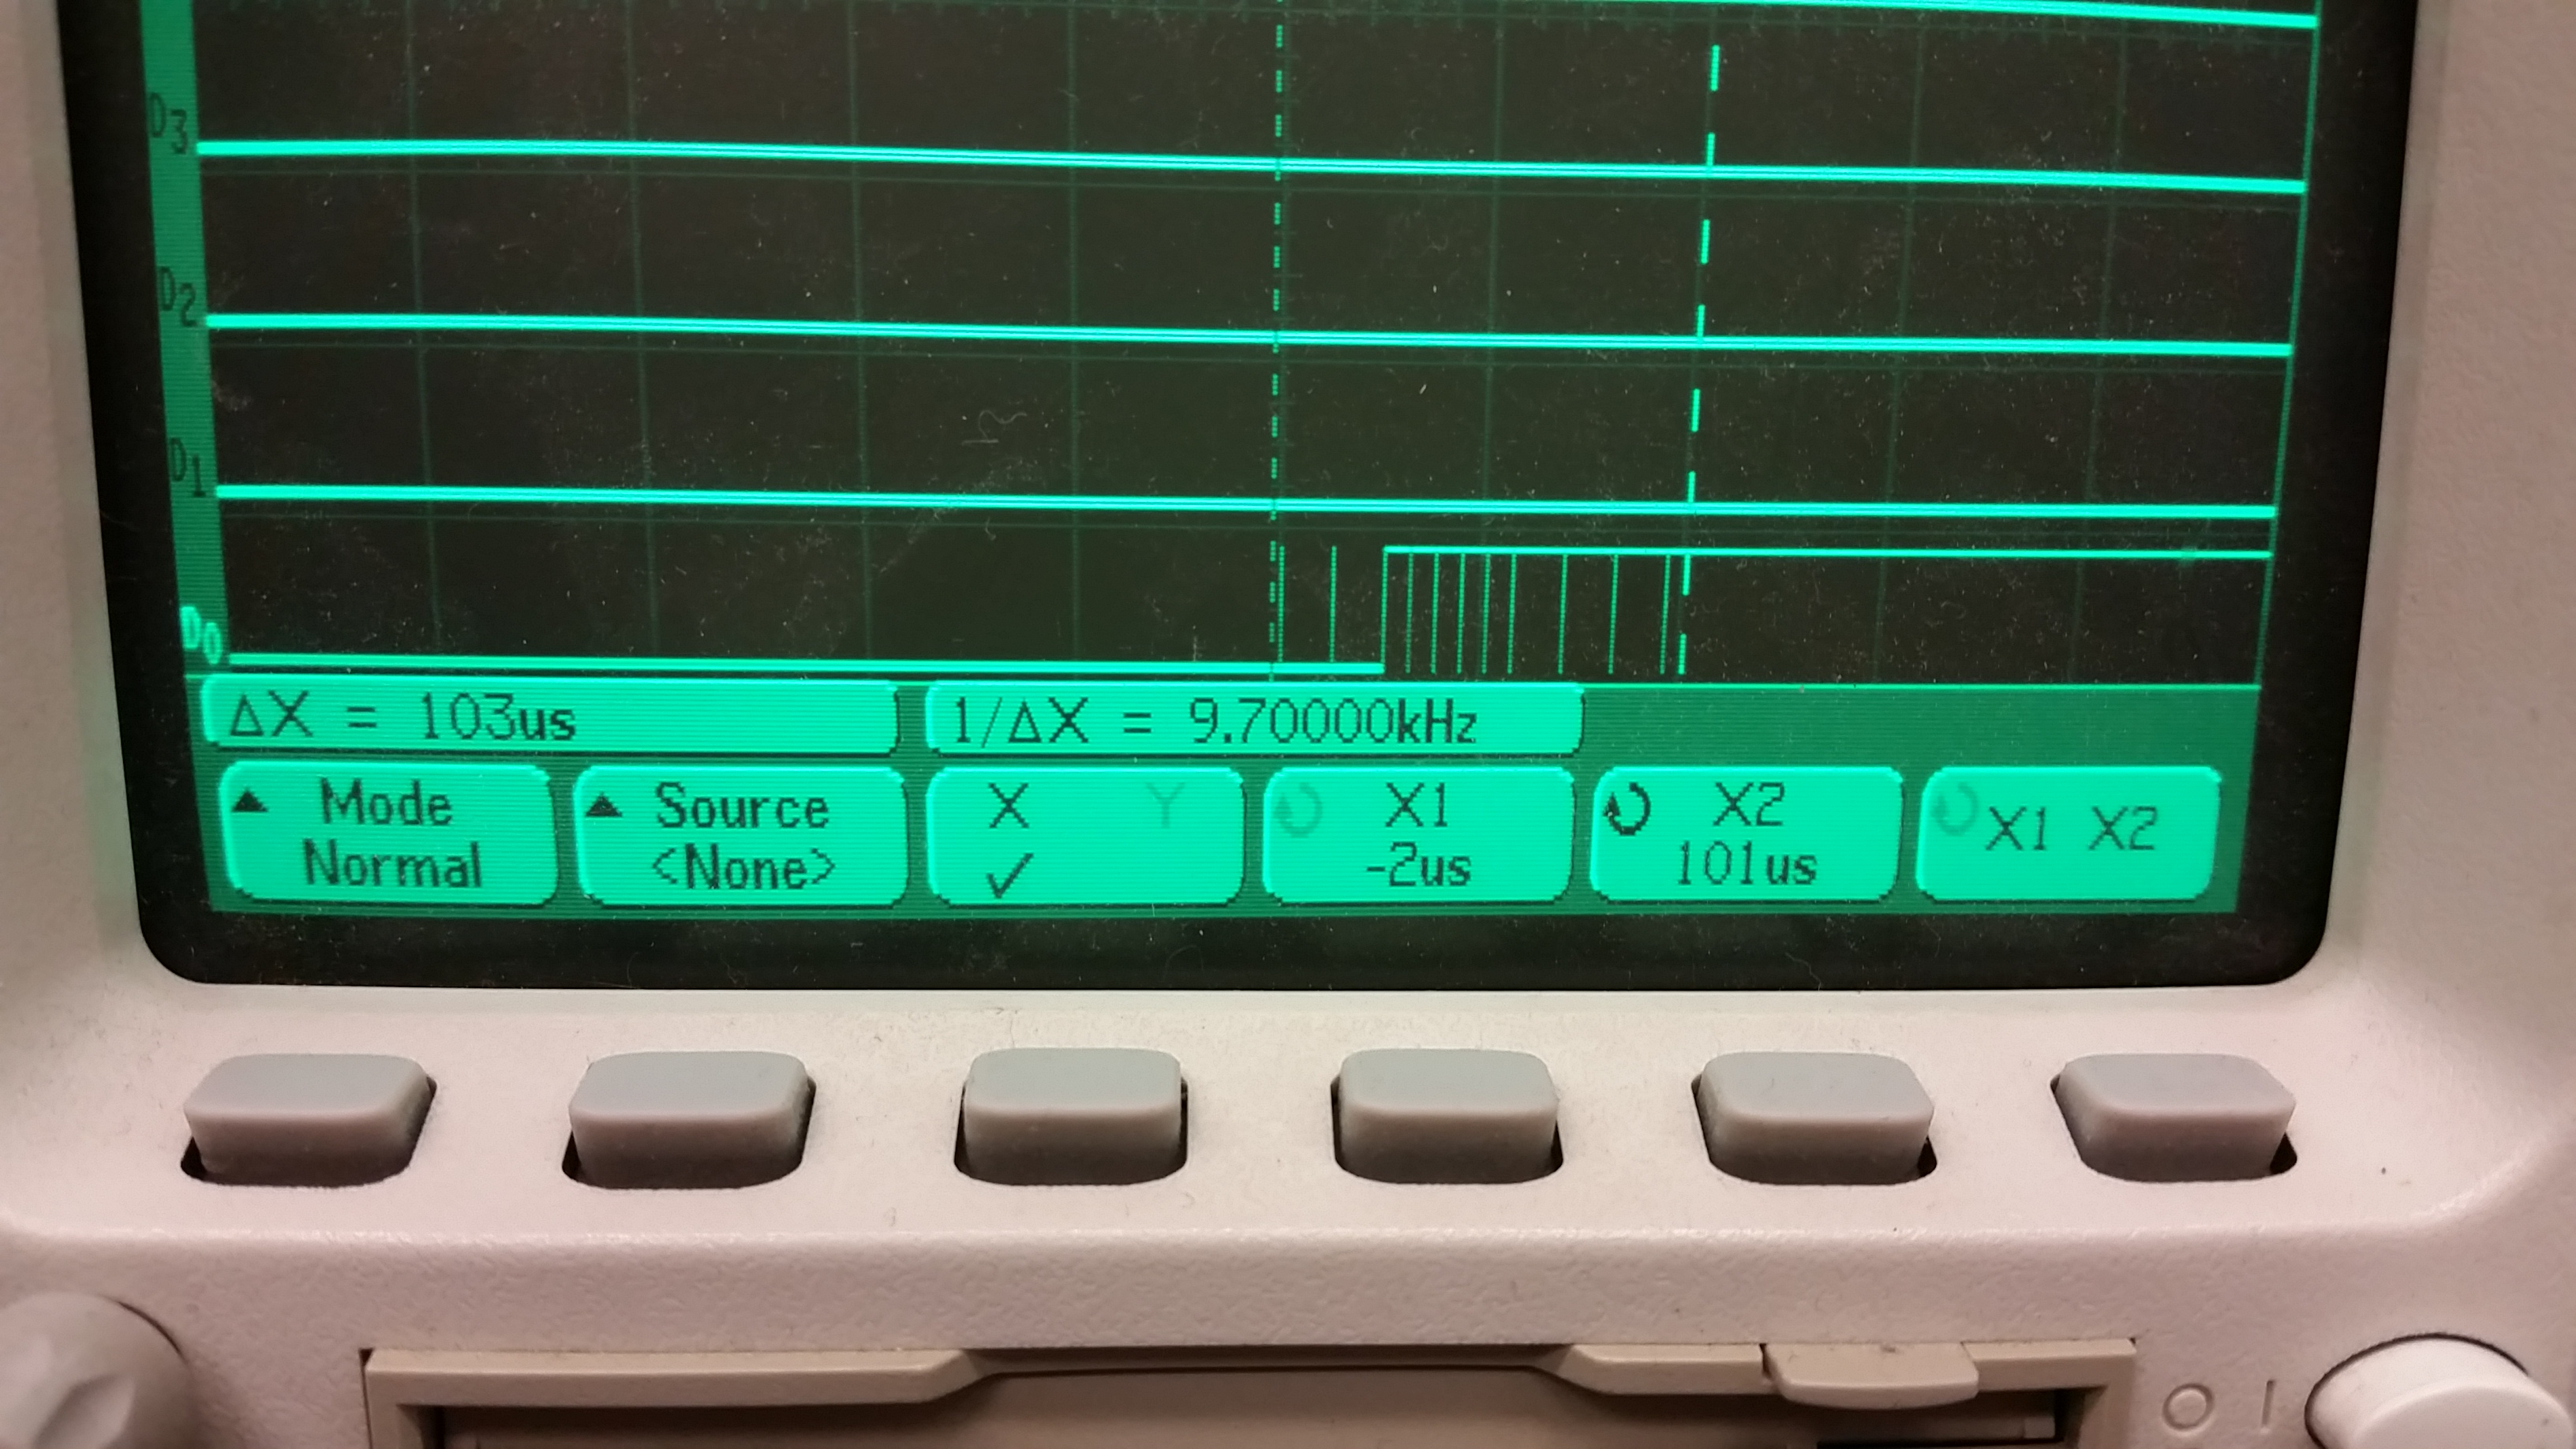
\includegraphics[scale=0.11]{bounce_rise.jpg}
\caption{Button bounce when the button is pressed down.}
\label{fig:bounce_rise}
\end{figure} 

\begin{figure}[h!]
\centering
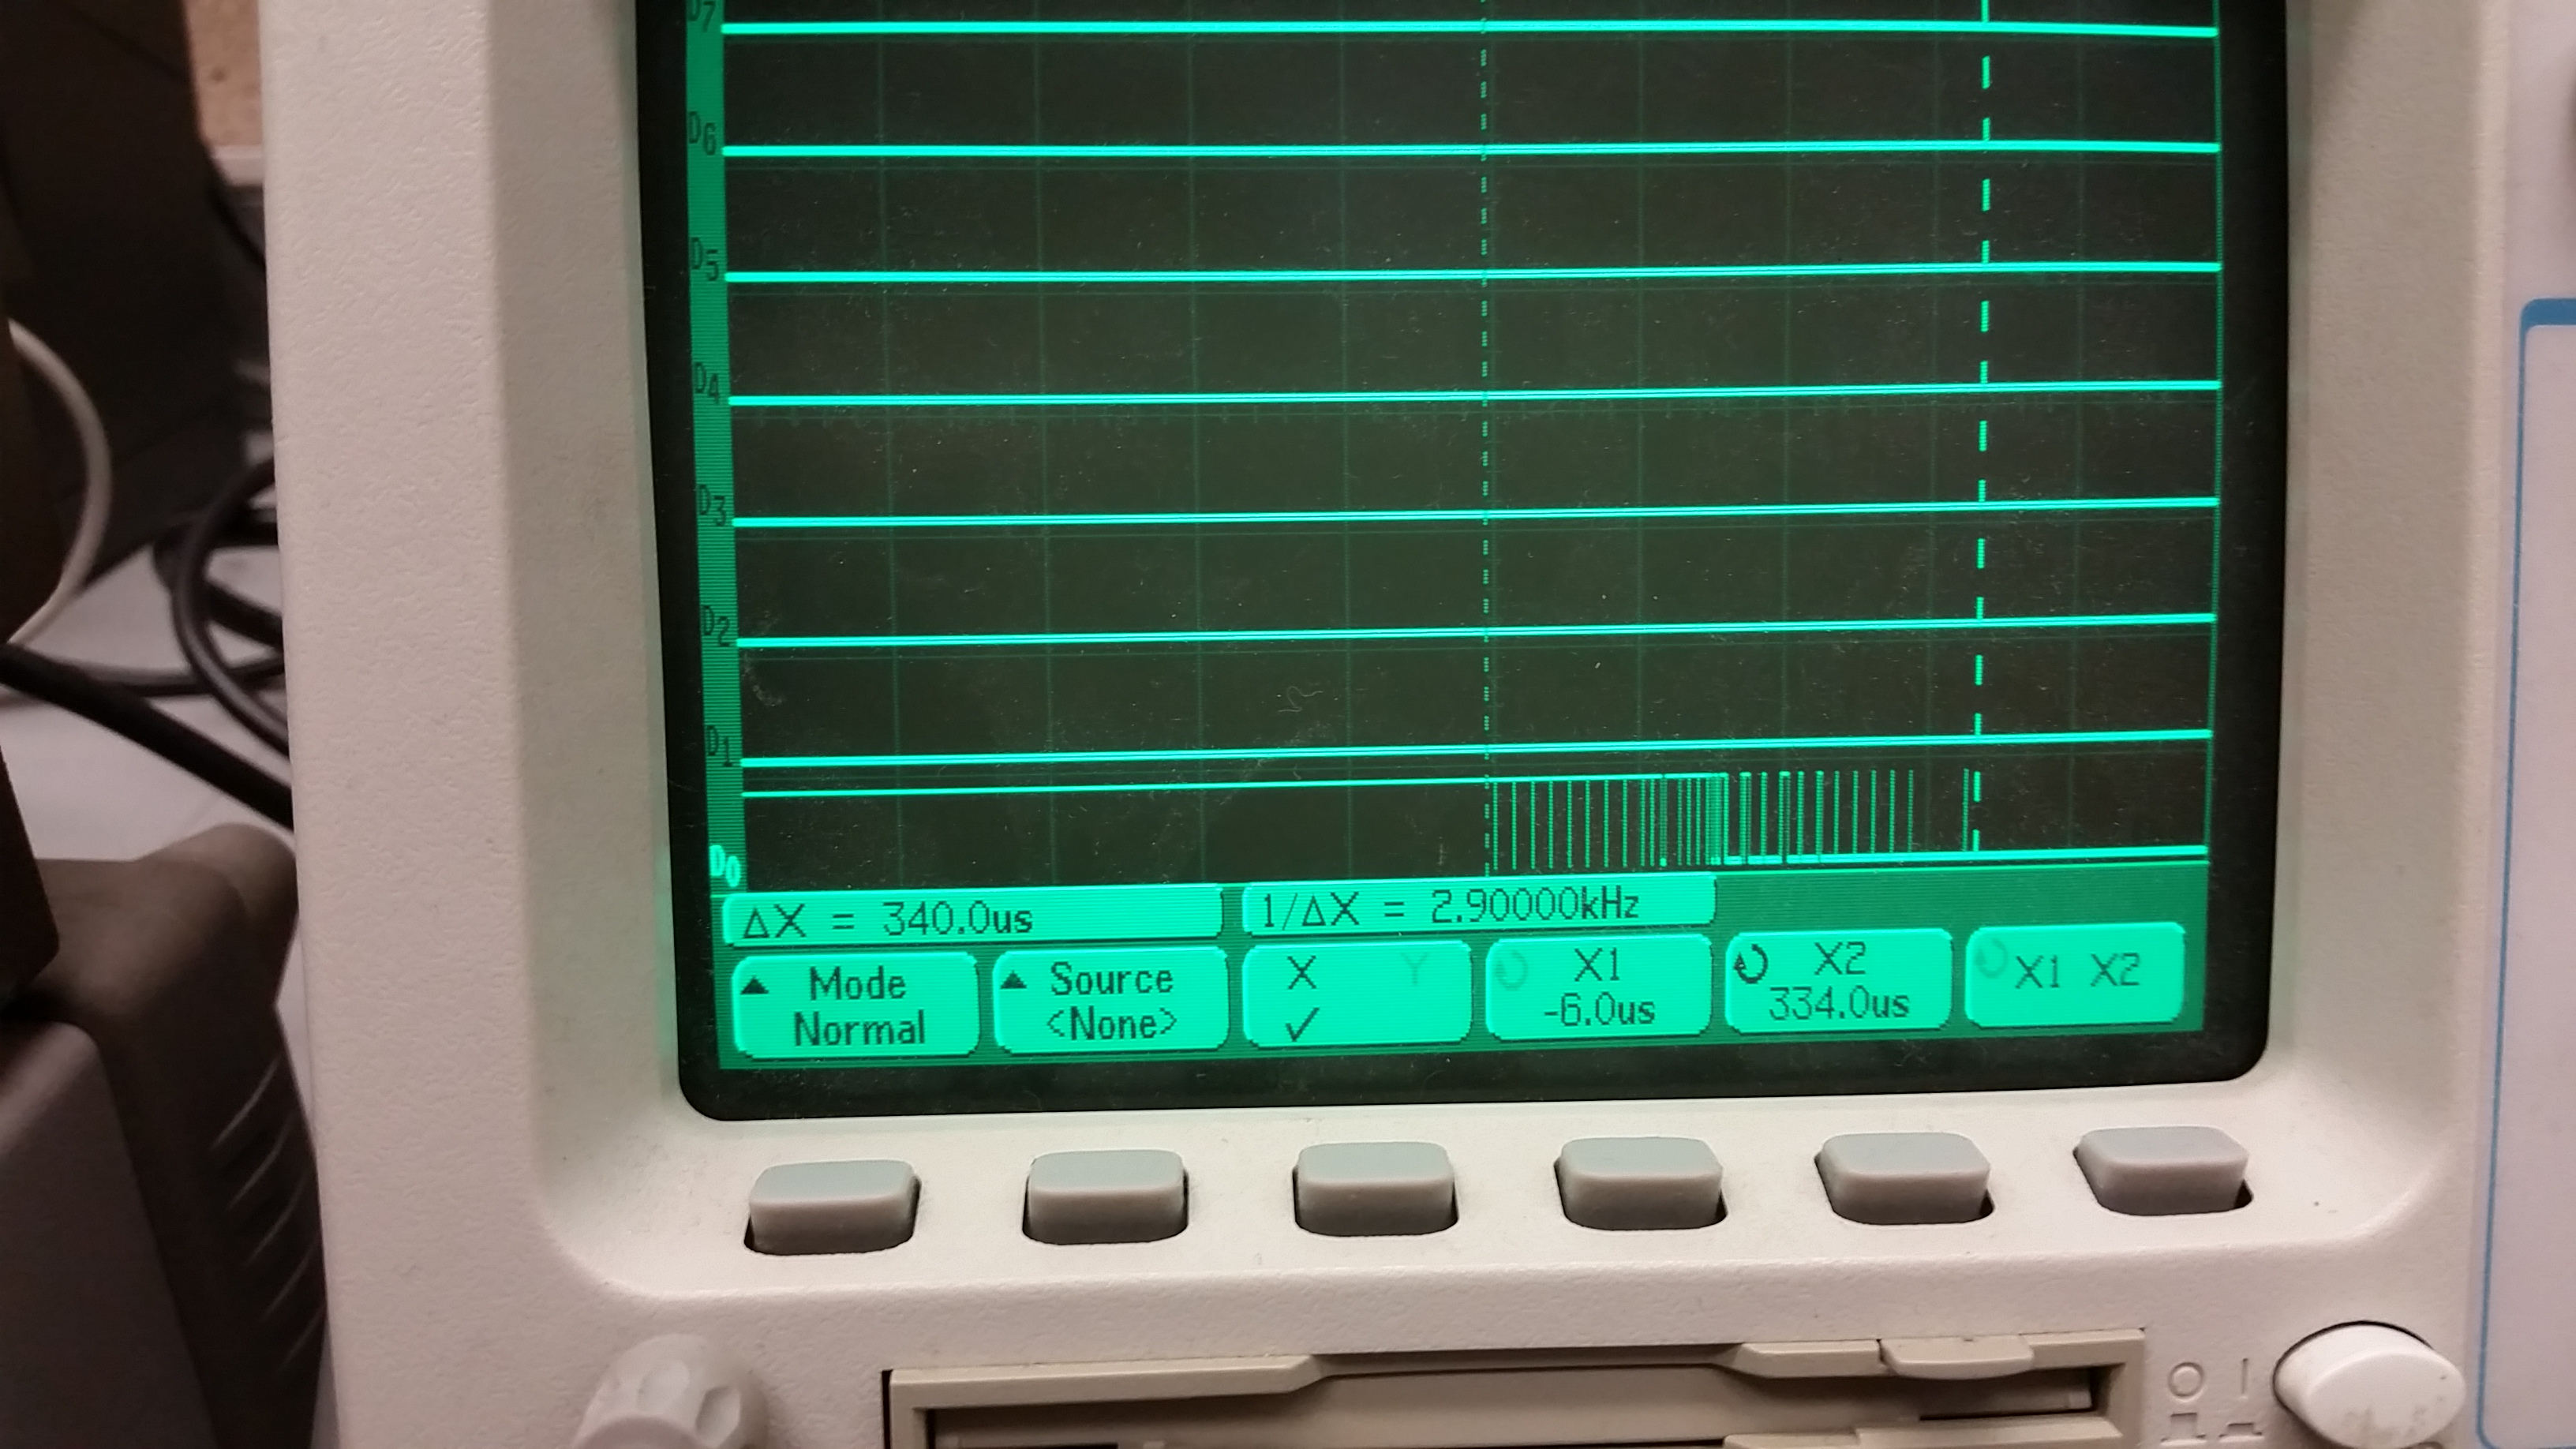
\includegraphics[scale=0.14]{bounce_fall.jpg}
\caption{Button bounce when the button is released.}
\label{fig:bounce_fall}
\end{figure} 



\subsection{Software}

The general approach to interpreting data from the keypad is as follows. First row 0 is powered. The column pins are read. If a button in that row is pressed down, the row remains powered until the button is released. If no button is pressed, row 0 is turned off and then row 1 is powered. Repeat. When button presses do occur, they are decoded based on the row being powered and the column that is read as HIGH. If multiple columns are HIGH at the same time, the left-most button is taken as the one being pressed down. \\

To cope with the challenge of button bounce, the control loop rate is run at a slow enough frequency to avoid sampling twice in the same button press. This means that if the button is sampled while the signal is bouncing as in Figure \ref{fig:bounce_rise}, either a HIGH or LOW will be sampled. However, the next sample will be taken after the signal has resolved to a steady value. So, to the controller no bouncing in the signal is visible. \\

From Figures \ref{fig:bounce_fall} and \ref{fig:bounce_rise}, I can see that longest observed button bounce duration is 340$\mu$s. So, the fastest the columns should be sampled at a particular row (accounting for a factor of safety of 2) is once every 680$\mu$s. Since there are 4 rows and I'm going to only sample the columns for a given row once every 4 samples, I can sample sequential rows at $\frac{680\mu s}{4}=170\mu s$. This corresponds with a frequency of 5.8kHz.

\begin{figure}[h!]
\centering
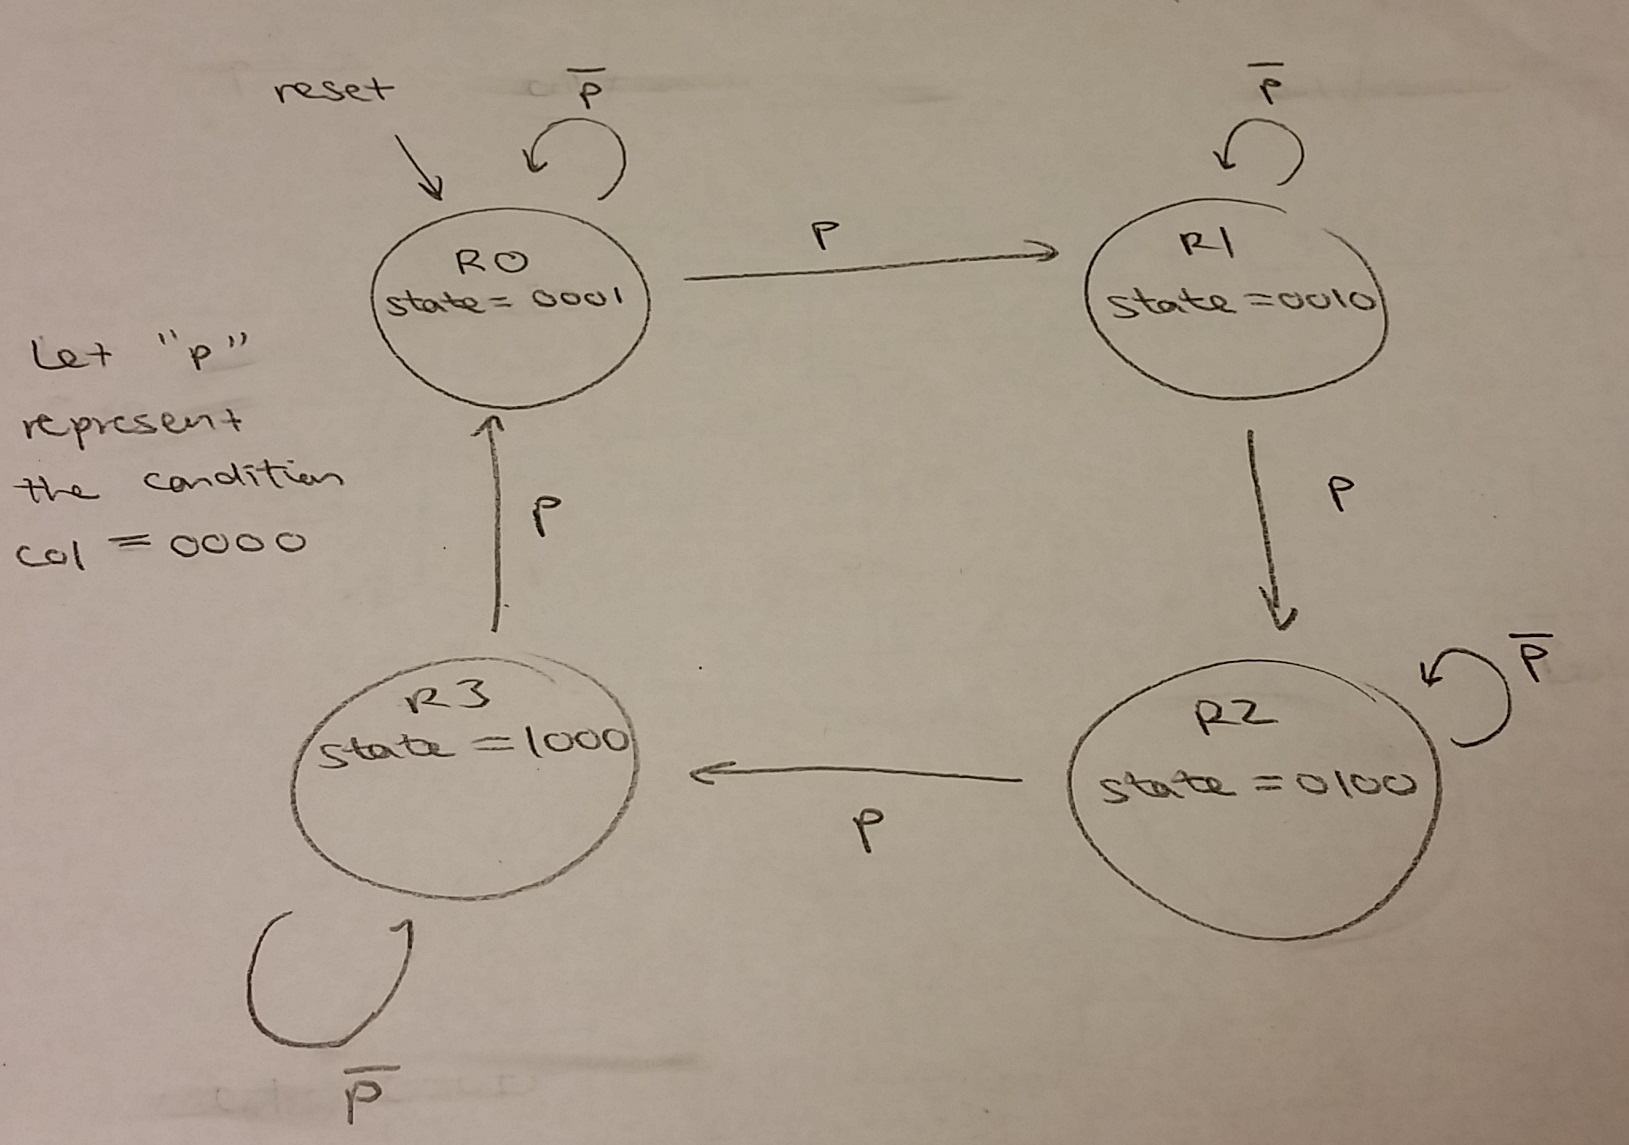
\includegraphics[scale=0.2]{fsm.jpg}
\caption{Finite state machine which keeps track of which row is being scanned.}
\label{fig:fsm}
\end{figure} 


\begin{figure}[h!]
\centering
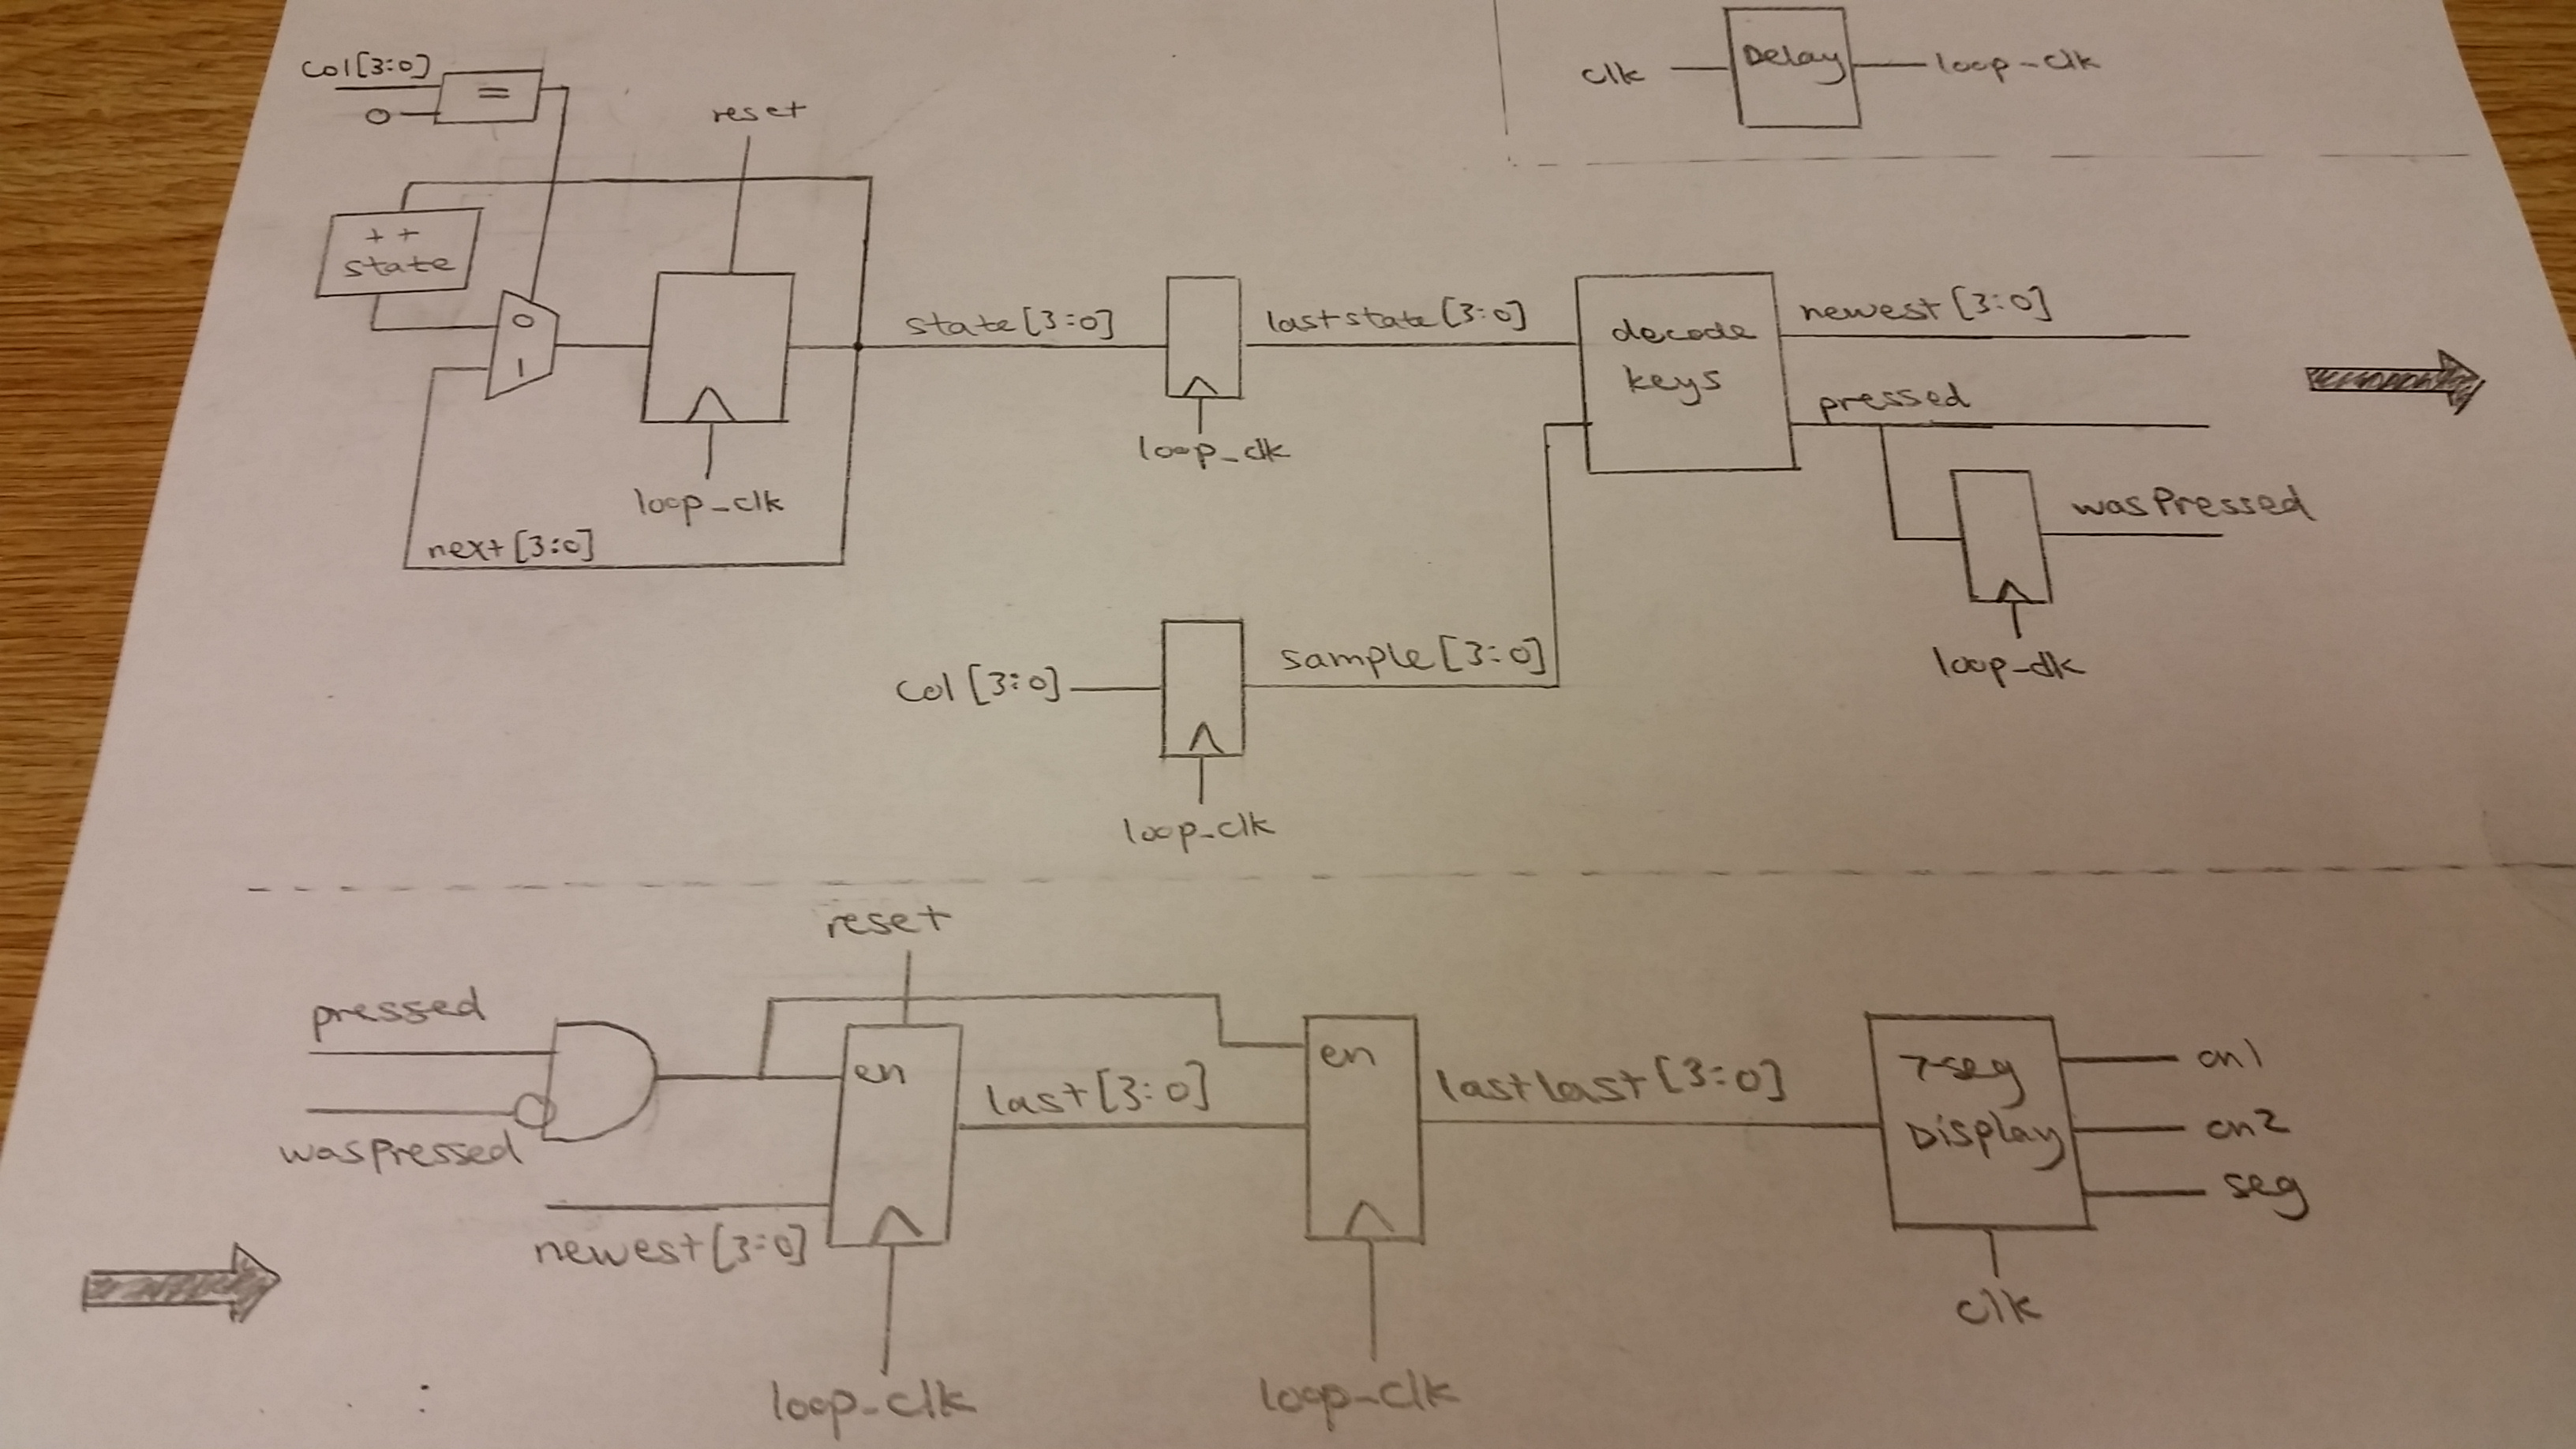
\includegraphics[scale=0.13]{flow.jpg}
\caption{Control flow of the program.}
\label{fig:flow}
\end{figure} 



\clearpage


\subsubsection{Simulation}

The code's logic was tested in ModelSim-Altera. The following show the results of the wave simulations that were run. The program was simulated in sections to ease debugging and wave simulation viewing.

\begin{figure}[h!]
\centering
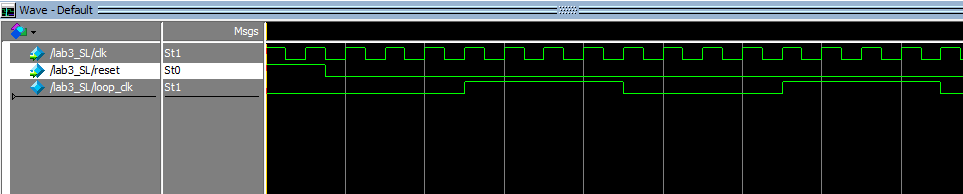
\includegraphics[scale=0.6]{subclk.png}
\caption{To slow the sampling rate of the program, a "loop clk" was created to run at a slower rate than the on board clk. All flip-flops in the design are run based on this this slower clock signal. Note that the loop clock in actuality runs much slower than what is shown.}
\label{fig:subclk}
\end{figure} 


\begin{figure}[h!]
\centering
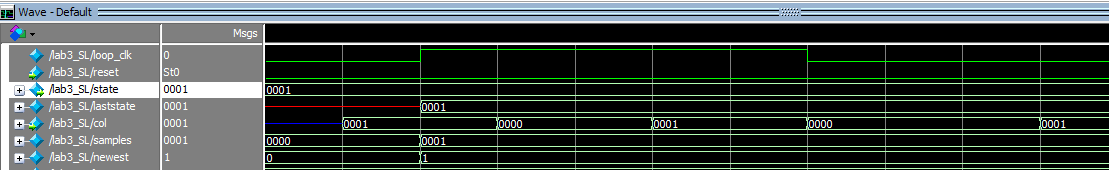
\includegraphics[scale=0.54]{bounce2.png}
\caption{Even if the columns signal bounces, only one sample is taken. Bounce does not appear in the control signal "newest." }
\label{fig:bounce}
\end{figure} 


\begin{figure}[h!]
\centering
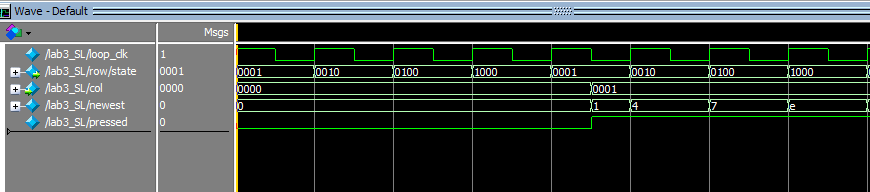
\includegraphics[scale=0.65]{keypad_decode.png}
\caption{The keypad decoder works! The signal state[3:0] gives the row that's being powered and col[3:0] gives which row is being powered. The hex symbol is on the signal "newest."}
\label{fig:keypad_decode}
\end{figure} 


\begin{figure}[h!]
\centering
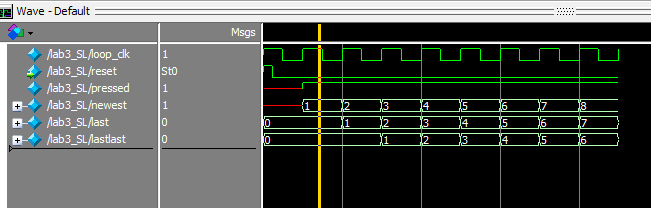
\includegraphics[scale=0.8]{mem.png}
\caption{The program accurately remembers the last two numbers. "last" is the latest number entered. "lastlast" is the second to last number entered.}
\label{fig:mem}
\end{figure} 


\begin{figure}[h!]
\centering
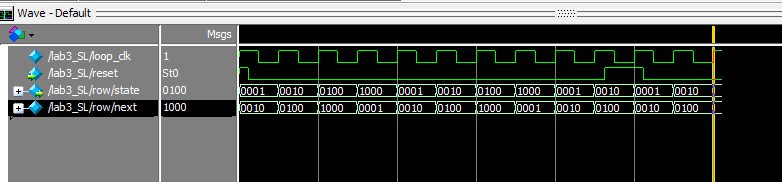
\includegraphics[scale=0.7]{rows.png}
\caption{The main finite-state-machine keeps track of which row is being powered. The state uses 1-hot encoding so that it can be directly routed to the output. "next" represents the next state. When the reset signal is pulled high, the state resets synchronously to 0001.}
\label{fig:states}
\end{figure} 


\begin{figure}[h!]
\centering
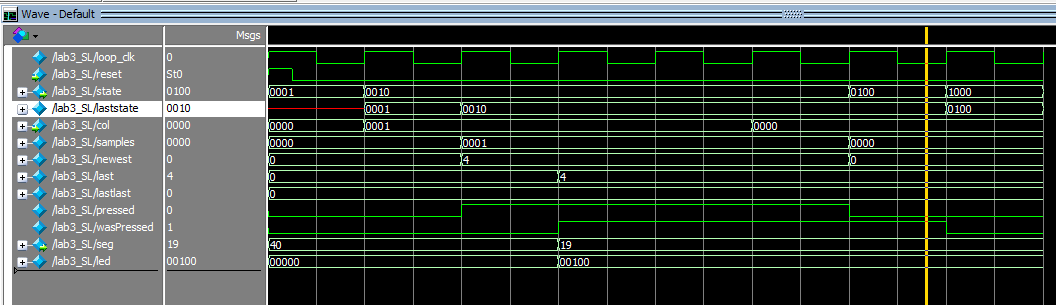
\includegraphics[scale=0.6]{state_change_on_button.png}
\caption{When a button is pressed, the FSM is frozen in its current state. This prevents the program from registering a button that's being held down as multiple button presses.}
\label{fig:button_held_down}
\end{figure} 



\clearpage

\section{Technical Documentation}

The following section shows schematics for the breadboard circuit that was built. The source code is also provided.

\subsection{7-Segment Decoder Truth Table}

\begin{table}[h]
\centering
\begin{tabular}{|c|c|c|c|c|c|c|c|c|c|c|c|c|}
\hline
\multicolumn{13}{|c|}{\textbf{7-Segment Display Truth Table}}                                  \\ \hline
\multicolumn{5}{|c|}{Inputs}                      & \multicolumn{8}{c|}{Ouputs}       \\ \hline
s3{[}3{]} & s3{[}2{]} & s3{[}1{]} & s3{[}0{]} & (hex) & G & F & E & D & C & B & A & (hex) \\ \hline
0        & 0        & 0        & 0        & 0x0   & 1 & 0 & 0 & 0 & 0 & 0 & 0 & 0x40  \\ \hline
0        & 0        & 0        & 1        & 0x1   & 1 & 1 & 1 & 1 & 0 & 0 & 1 & 0x79  \\ \hline
0        & 0        & 1        & 0        & 0x2   & 0 & 1 & 0 & 0 & 1 & 0 & 0 & 0x24  \\ \hline
0        & 0        & 1        & 1        & 0x3   & 0 & 1 & 1 & 0 & 0 & 0 & 0 & 0x30  \\ \hline
0        & 1        & 0        & 0        & 0x4   & 0 & 0 & 1 & 1 & 0 & 0 & 1 & 0x19  \\ \hline
0        & 1        & 0        & 1        & 0x5   & 0 & 0 & 1 & 0 & 0 & 1 & 0 & 0x12  \\ \hline
0        & 1        & 1        & 0        & 0x6   & 0 & 0 & 0 & 0 & 0 & 1 & 0 & 0x02  \\ \hline
0        & 1        & 1        & 1        & 0x7   & 1 & 1 & 1 & 1 & 0 & 0 & 0 & 0x78  \\ \hline
1        & 0        & 0        & 0        & 0x8   & 0 & 0 & 0 & 0 & 0 & 0 & 0 & 0x00  \\ \hline
1        & 0        & 0        & 1        & 0x9   & 0 & 0 & 1 & 1 & 0 & 0 & 0 & 0x18  \\ \hline
1        & 0        & 1        & 0        & 0xA   & 0 & 0 & 0 & 1 & 0 & 0 & 0 & 0x08  \\ \hline
1        & 0        & 1        & 1        & 0xB   & 0 & 0 & 0 & 0 & 0 & 1 & 1 & 0x03  \\ \hline
1        & 1        & 0        & 0        & 0xC   & 0 & 1 & 0 & 0 & 1 & 1 & 1 & 0x27  \\ \hline
1        & 1        & 0        & 1        & 0xD   & 0 & 1 & 0 & 0 & 0 & 0 & 1 & 0x21  \\ \hline
1        & 1        & 1        & 0        & 0xE   & 0 & 0 & 0 & 0 & 1 & 1 & 0 & 0x06  \\ \hline
1        & 1        & 1        & 1        & 0xF   & 0 & 0 & 0 & 1 & 1 & 1 & 0 & 0x0E  \\ \hline
\end{tabular}
\caption{Truth table for 7-Segment LED decoder}
\label{table:7seg_decoder}
\end{table}


\subsection{7-segment Displays Schematic}


\begin{figure}[h!]
\centering
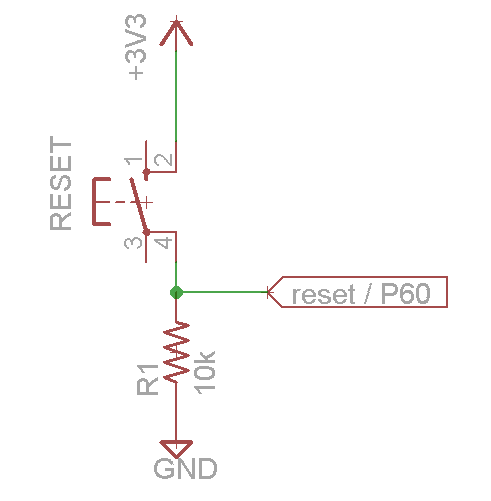
\includegraphics[scale=0.54]{reset.png}
\caption{Schematic for reset button.}
\label{fig:reset_sch}
\end{figure} 


\begin{figure}[h!]
\centering
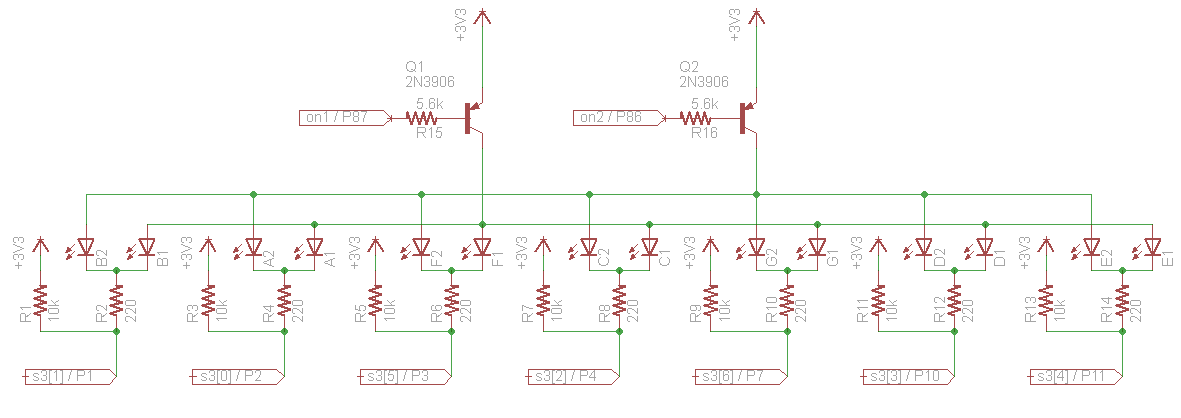
\includegraphics[scale=0.7, angle=90]{seven_segment_all.png}
\caption{Full schematic for dual 7-segment display. Note that on1 and on2 toggle the two displays on and off. Only one or the other is on at any given time.}
\label{fig:seven_seg_sch}
\end{figure} 


\clearpage

\subsection{Pin Mapping}

\begin{table}[h!]
\centering
\begin{tabular}{|c|c|c|c|}
\hline
\multicolumn{4}{|c|}{\textbf{Keypad Pin Mapping - Rows}}                                                                                                     \\ \hline
R0 / state{[}0{]} & R1 / state{[}1{]} & R2 / state{[}2{]} & R3 / state{[}3{]} \\ \hline
P70               & P66               & P67               & P69               \\ \hline
\end{tabular}
\caption{Pin mapping of keypad - Rows}
\label{table:pinmap_keypad_row}
\end{table}


\begin{table}[h!]
\centering
\begin{tabular}{|c|c|c|c|}
\hline
\multicolumn{4}{|c|}{\textbf{Keypad Pin Mapping - Columns}}                                                                                                     \\ \hline
C0 / col{[}0{]} & C1 / col{[}1{]} & C2 / col{[}2{]} & C3 / col{[}3{]} \\ \hline
P68             & P73             & P72             & P71             \\ \hline
\end{tabular}
\caption{Pin mapping of keypad}
\label{table:pinmap_keypad_col}
\end{table}

\begin{table}[h!]
\centering
\begin{tabular}{|c|c|c|c|}
\hline
\multicolumn{4}{|c|}{\textbf{Control Signals Pin Mapping}} \\ \hline
on1        & on2        & clk        & reset       \\ \hline
P87        & P86        & P88        & P60         \\ \hline
\end{tabular}
\caption{Pin mapping of control signals}
\label{table:pinmap_control}
\end{table}

\begin{table}[h!]
\centering
\begin{tabular}{|c|c|c|c|c|c|c|}
\hline
\multicolumn{7}{|c|}{\textbf{7 - Segment Display Pin Mapping}} \\ \hline
seg[0]/A   & seg[1]/B   & seg[3]/C   & seg[4]/D    & seg[5]/E    & seg[6]/F   & seg[7]/G   \\ \hline
P2         & P1         & P4         & P10         & P11         & P3         & P7  \\ \hline
\end{tabular}
\caption{Pin mapping of 7-segment display}
\label{table:pinmap_sevenseg}
\end{table}



\clearpage
\subsection{System Verilog Code}

\subsubsection{Controller}

\begin{lstlisting}[language=Verilog,numbers=left,basicstyle=\footnotesize]
/* This is the project wrapper that inits all the
individual components of the project

Author: Sherman Lam
Email: slam@g.hmc.edu
Date: Sep 25, 2014
*/
module lab3_SL(   input logic clk, reset,
                  input logic [3:0] col,
                  output logic on1,on2,
                  output logic [3:0] state,
                  output logic [6:0] seg);
   //wires
   logic[3:0] newest;
   logic[3:0] last;
   logic[3:0] lastlast;
   logic pressed;
   logic wasPressed;
   logic loop_clk;
   logic[4:0] led;
   logic[3:0] samples;
   logic[3:0] laststate;
   
   // run the clk at a slower rate
   clk_sm         subClk(  .clk(clk),
                           .reset(reset),
                           .loop_clk(loop_clk));  
   
   //keep track of the last 2 numbers
   record_sm      memory(  .loop_clk(loop_clk),
                           .reset(reset),
                           .pressed(pressed),
                           .newest(newest),
                           .last(last),
                           .lastlast(lastlast),
                           .wasPressed(wasPressed));
   
   //fsm for deciding which row to check next
   row_sm         row(  .loop_clk(loop_clk),
                        .reset(reset),
                        .state(state),
                        .col(col));
   
   //sample the keys synchronously
   sample_keys    sample(  .loop_clk(loop_clk),
                           .reset(reset),
                           .col(col),
                           .samples(samples));
   
   //remember the last state
   last_state     rememberState( .loop_clk(loop_clk),
                                 .state(state),
                                 .laststate(laststate));
   
   //read the rows and cols of the keypad and decode to hex
   decode_keys    read( .laststate(laststate),
                        .samples(samples),
                        .pressed(pressed),
                        .newest(newest));

   // keeps track if key was pressed in the last time step
   record_pressed recordPressed( .loop_clk(loop_clk),
                                 .reset(reset),
                                 .pressed(pressed),
                                 .wasPressed(wasPressed));
   
   //seven segment display
   seven_seg_displays      seven_seg(.clk(clk),.reset(reset),.s1(lastlast),
                              .s2(last),.on1(on1),.on2(on2),.seg(seg),
                              .led(led));
            
endmodule


/* This keeps track of the last state

Author: Sherman Lam
Email: slam@g.hmc.edu
Date: Sep 27, 2014
*/
module last_state(input logic loop_clk,
                  input logic [3:0] state,
                  output logic [3:0] laststate);
      always_ff@(posedge loop_clk) begin
         laststate <= state;
      end
endmodule


/* This is a state machine that is used to keep
track of which row is being checked

Author: Sherman
Email: slam@g.hmc.edu
Date: Sep 25,2104
*/
module row_sm( input logic loop_clk, reset,
               input logic [3:0] col,
               output logic [3:0] state);
   
   //state encodings
   parameter ROW1 = 4'b0001;
   parameter ROW2 = 4'b0010;
   parameter ROW3 = 4'b0100;
   parameter ROW4 = 4'b1000;
   
   //next state
   logic [3:0] next;
   
   always_ff@(posedge loop_clk) begin
      if (reset)
         state <= ROW1;
      else if (col == 4'b0000)      //only switch rows when button not pressed.
         state <= next;
      else  
         state <= state;   
      
   end         
   
   always_comb begin
      //next state logic
      case (state)
         ROW1:       next = ROW2;
         ROW2:       next = ROW3;
         ROW3:       next = ROW4;
         ROW4:       next = ROW1;
         default:    next = ROW1;
      endcase
   end
   
endmodule


/* This samples the keys at the rising edge of loop_clk.
This is meant to prevent button bounce.

Author: Sherman Lam
Email: slam@g.hmc.edu
Date: Sep 26,2014
*/
module sample_keys(  input logic loop_clk, reset,
                     input logic [3:0] col, 
                     output logic [3:0] samples);
      always_ff@(posedge loop_clk) begin
         if (reset)
            samples <= 4'b0000;
         else begin
            samples <= col;
         end
      end
endmodule


/* This checks whether or not a button has been pressed.

Author: Sherman Lam
Email: slam@g.hmc.edu
Date: Sep 25, 2014
*/
module decode_keys(  input logic [3:0] laststate,
                  input logic [3:0] samples,
                  output logic pressed,
                  output logic [3:0] newest);
   logic [4:0] key = 'b0;
   always_comb begin
      //check each row
      case(laststate)
         4'b0001: casez(samples)       // find the first key
                  4'b1???: key = 5'hA;
                  4'b01??: key = 5'h3;
                  4'b001?: key = 5'h2;
                  4'b0001: key = 5'h1;
                  default: key = 5'h10;   // no key      
               endcase  
         4'b0010: casez(samples)       // find the first key
                  4'b1???: key = 5'hB;
                  4'b01??: key = 5'h6;
                  4'b001?: key = 5'h5;
                  4'b0001: key = 5'h4;
                  default: key = 5'h10;   // no key      
               endcase  
         4'b0100: casez(samples)       // find the first key
                  4'b1???: key = 5'hC;
                  4'b01??: key = 5'h9;
                  4'b001?: key = 5'h8;
                  4'b0001: key = 5'h7;
                  default: key = 5'h10;   // no key      
               endcase        
         4'b1000: casez(samples)       // find the first key
                  4'b1???: key = 5'hD;
                  4'b01??: key = 5'hF;
                  4'b001?: key = 5'h0;
                  4'b0001: key = 5'hE;
                  default: key = 5'h10;   // no key      
               endcase  
         default:          key = 5'h10;
      endcase
      
      //key is only pressed if we found a key
      pressed = ~key[4];
      newest = key[3:0];
      
      //TODO: change pressed to also depend on the state. Store pressed
      // as a 4 bit number.
   
   end
endmodule
      
               
/* This keeps track of whether or not a key was pressed in
the last time step

Author: Sherman Lam
Email: slam@g.hmc.edu
Date: Sep 25, 2014
*/
module record_pressed(  input logic pressed, loop_clk, reset,
                     output logic wasPressed);
      always_ff@(posedge loop_clk) begin
         if (reset == 1'b1)
            wasPressed = 1'b0;
         else
            wasPressed <= pressed;
      end
   
endmodule   


/* This is a state machine that sorts the presses

Author: Sherman Lam
Email: slam@g.hmc.edu
Date: Sep 27, 2014
*/


/* This is the state machine that records the last
two values (last and lastlast) entered into the keypad. 

Author: Sherman
Email: slam@g.hmc.edu
Date: Sep 25,2104
*/
module record_sm( input logic loop_clk, reset,
                  input logic pressed, wasPressed,
                  input logic [3:0] newest,
                  output logic [3:0] last, lastlast);
   // store
   always_ff@(posedge loop_clk, posedge reset) begin
      if (reset) begin
         last = 'h0;
         lastlast = 'h0; 
      end
      //record only the first instance of the press
      else if (pressed & (~wasPressed)) begin
         lastlast <= last;
         last <= newest;
      end
      else begin
         lastlast <= lastlast;
         last <= last;
      end
   end
endmodule


/* This is the state machine that outputs a slower
clk. This allows the program to run at a slower control
loop rate than that of the on board clock.

debounce math: 
Scanning 1 row max: 2.9kHz
Scanning 1 row with FOS of 2: 1.45kHz
Scanning 4 rows: 5.8kHz
Loop every 6897 clock cycles
Toggle clk every 3448 clock cycles


Author: Sherman
Email: slam@g.hmc.edu
Date: Sep 25,2104
*/
module clk_sm( input logic clk, reset,
               output logic loop_clk);

parameter HALF_PERIOD = 28'd3448; //5.9kHz loop rate
logic [27:0] counter = '0;

always_ff@(posedge clk, posedge reset) begin
   if (reset == 1'b1) begin               
      counter = '0;
      loop_clk = 0;
   end
   else if (counter >= HALF_PERIOD) begin
      counter = '0;
      loop_clk = ~loop_clk;      //toggle loop_clk
   end
   else begin
      counter = counter + 1'b1;
      loop_clk = loop_clk;
   end
end


endmodule

\end{lstlisting}


\subsubsection{7-segment display}

\begin{lstlisting}[language=Verilog,numbers=left,basicstyle=\footnotesize]
/* This is the main module. It selects which set of switch
   outputs to use and then decodes the number of the selected
   switch. This also sets the clock that time-multiplexes the 
   two 7 segment outputs.
   
   Author: Sherman Lam
   Email: slam@g.hmc.edu
   Date: Sep 17, 2014
*/
module seven_seg_displays(input logic clk, reset,
               input logic [3:0] s1,s2, //DIP switches
               output logic on1, on2,   //if on1 is pulled LOW, LED set 1 is on.
               output logic [6:0] seg,
               output logic [4:0] led); //segment states    
   
   // time multiplexing
   multiplexer m1(.clk(clk), .on1(on1), .reset(reset));
   
   // the segments always have opposite states.
   assign on2 = ~on1;      
   
   // select the right set of switches.
   // on1 -> s1 is used. on2 -> s2 is used
   // if on1 is pulled LOW, LED set 1 is on.
   logic [3:0] s3;
   assign s3 = on1? s2 : s1;  
   
   // 7 segment decoder
   led7Decoder decoder(.s(s3), .seg(seg));
   
   // sum the outputs and write to LED bar
   assign led = s1 + s2;
   
   
endmodule


/* This module time multiplexes

   Author: Sherman Lam
   Email: slam@g.hmc.edu
   Date: Sep 17, 2014
*/
module multiplexer(  input logic clk, reset,
                     output logic on1);
   // time multiplexer for switching between displays
   logic [18:0] hPeriod = 19'd333333;  // 120Hz toggling
   logic [18:0] counter = 'b0;
      
   always_ff @(posedge clk, posedge reset) begin
      if (reset)     
         on1 = 1'b0;
      else begin
         if (counter >= hPeriod) begin
            counter = 'b0;
            on1 = ~on1;
         end
         else
            //on1 = on1;
            counter <= counter + 1'b1;
      end
   end
   
endmodule


/* This module decodes the switch inputs into an output for the 
   7 segment display on the development board.
   s[3:0] = [sw3, ... ,sw1]
   seg[6:0] = [g,f, ... ,b,a]
   
   Author: Sherman
   Email: slam@g.hmc.edu
   Date: Sep 9, 2014
*/
module led7Decoder(  input logic [3:0] s,       //4 DIP switches
                     output logic [6:0] seg);   //segments in 7-seg display
                     
   always_comb begin
      //lookup table for s-seg relationship
      case(s)
         4'h0: seg = 7'b100_0000;      // 0x0
         4'h1: seg = 7'b111_1001;      // 0x1
         4'h2: seg = 7'b010_0100;      // 0x2
         4'h3: seg = 7'b011_0000;      // 0x3
         4'h4: seg = 7'b001_1001;      // 0x4
         4'h5: seg = 7'b001_0010;      // 0x5
         4'h6: seg = 7'b000_0010;      // 0x6
         4'h7: seg = 7'b111_1000;      // 0x7
         4'h8: seg = 7'b000_0000;      // 0x8
         4'h9: seg = 7'b001_1000;      // 0x9
         4'ha: seg = 7'b000_1000;      // 0xA
         4'hb: seg = 7'b000_0011;      // 0xB
         4'hc: seg = 7'b010_0111;      // 0xC
         4'hd: seg = 7'b010_0001;      // 0xD
         4'he: seg = 7'b000_0110;      // 0xE
         4'hf: seg = 7'b000_1110;      // 0xF
         default: seg = 7'b111_1110;      // default to a dash
      endcase
      
   end
endmodule
\end{lstlisting}



\clearpage

\section{Results and Discussion}

The system works as expected and can handle rapid key sequences without freezing. If at any point the user desires to clear the numbers, a reset button is available that resets the displays to 0.

\section{Conclusion}

\subsection{Time Spent}

\begin{description}
	\item[Programming, Simulating] 13hrs
	\item[Breadboarding] 0.5hrs
	\item[Writing Report] 5hrs
	\item[Total Time Spent] 18.5hrs
\end{description}

\subsection{Suggestions for lab}

None. Very challenging.


\end{document}

